\documentclass[tikz,border=5pt]{standalone}
\usepackage{amsmath,amssymb}
\usetikzlibrary{arrows.meta}
\definecolor{curveblue}{HTML}{245C86}
\definecolor{accent}{HTML}{A65E2E}
\begin{document}
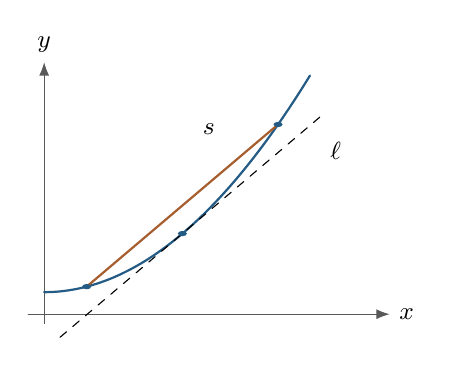
\begin{tikzpicture}[font=\small,>=Latex,line cap=round,line join=round]
\begin{scope}[shift={(0.00000,0.00000)},xscale=1.35,yscale=0.8]
\draw[->,black!65] (-0.15000,0.00000)--(3.25000,0.00000);
\node[right] at (3.25000,0.00000) {$x$};
\draw[->,black!65] (0.00000,-0.15000)--(0.00000,4.00000);
\node[above] at (0.00000,4.00000) {$y$};
\draw[curveblue,thick] plot[smooth] coordinates {(0.00000,0.35000) (0.01667,0.35015) (0.03333,0.35061) (0.05000,0.35137) (0.06667,0.35244) (0.08333,0.35382) (0.10000,0.35550) (0.11667,0.35749) (0.13333,0.35978) (0.15000,0.36238) (0.16667,0.36528) (0.18333,0.36849) (0.20000,0.37200) (0.21667,0.37582) (0.23333,0.37994) (0.25000,0.38437) (0.26667,0.38911) (0.28333,0.39415) (0.30000,0.39950) (0.31667,0.40515) (0.33333,0.41111) (0.35000,0.41737) (0.36667,0.42394) (0.38333,0.43082) (0.40000,0.43800) (0.41667,0.44549) (0.43333,0.45328) (0.45000,0.46137) (0.46667,0.46978) (0.48333,0.47849) (0.50000,0.48750) (0.51667,0.49682) (0.53333,0.50644) (0.55000,0.51638) (0.56667,0.52661) (0.58333,0.53715) (0.60000,0.54800) (0.61667,0.55915) (0.63333,0.57061) (0.65000,0.58237) (0.66667,0.59444) (0.68333,0.60682) (0.70000,0.61950) (0.71667,0.63249) (0.73333,0.64578) (0.75000,0.65938) (0.76667,0.67328) (0.78333,0.68749) (0.80000,0.70200) (0.81667,0.71682) (0.83333,0.73194) (0.85000,0.74738) (0.86667,0.76311) (0.88333,0.77915) (0.90000,0.79550) (0.91667,0.81215) (0.93333,0.82911) (0.95000,0.84637) (0.96667,0.86394) (0.98333,0.88182) (1.00000,0.90000) (1.01667,0.91849) (1.03333,0.93728) (1.05000,0.95638) (1.06667,0.97578) (1.08333,0.99549) (1.10000,1.01550) (1.11667,1.03582) (1.13333,1.05644) (1.15000,1.07737) (1.16667,1.09861) (1.18333,1.12015) (1.20000,1.14200) (1.21667,1.16415) (1.23333,1.18661) (1.25000,1.20938) (1.26667,1.23244) (1.28333,1.25582) (1.30000,1.27950) (1.31667,1.30349) (1.33333,1.32778) (1.35000,1.35238) (1.36667,1.37728) (1.38333,1.40249) (1.40000,1.42800) (1.41667,1.45382) (1.43333,1.47994) (1.45000,1.50637) (1.46667,1.53311) (1.48333,1.56015) (1.50000,1.58750) (1.51667,1.61515) (1.53333,1.64311) (1.55000,1.67138) (1.56667,1.69994) (1.58333,1.72882) (1.60000,1.75800) (1.61667,1.78749) (1.63333,1.81728) (1.65000,1.84737) (1.66667,1.87778) (1.68333,1.90849) (1.70000,1.93950) (1.71667,1.97082) (1.73333,2.00244) (1.75000,2.03438) (1.76667,2.06661) (1.78333,2.09915) (1.80000,2.13200) (1.81667,2.16515) (1.83333,2.19861) (1.85000,2.23238) (1.86667,2.26644) (1.88333,2.30082) (1.90000,2.33550) (1.91667,2.37049) (1.93333,2.40578) (1.95000,2.44137) (1.96667,2.47728) (1.98333,2.51349) (2.00000,2.55000) (2.01667,2.58682) (2.03333,2.62394) (2.05000,2.66137) (2.06667,2.69911) (2.08333,2.73715) (2.10000,2.77550) (2.11667,2.81415) (2.13333,2.85311) (2.15000,2.89238) (2.16667,2.93194) (2.18333,2.97182) (2.20000,3.01200) (2.21667,3.05249) (2.23333,3.09328) (2.25000,3.13438) (2.26667,3.17578) (2.28333,3.21749) (2.30000,3.25950) (2.31667,3.30182) (2.33333,3.34444) (2.35000,3.38738) (2.36667,3.43061) (2.38333,3.47415) (2.40000,3.51800) (2.41667,3.56215) (2.43333,3.60661) (2.45000,3.65138) (2.46667,3.69644) (2.48333,3.74182) (2.50000,3.78750)};
\draw[accent,thick] (0.40000,0.43800)--(2.20000,3.01200);
\draw[black,dashed] plot[smooth] coordinates {(0.15000,-0.36500) (0.16667,-0.34117) (0.18333,-0.31733) (0.20000,-0.29350) (0.21667,-0.26967) (0.23333,-0.24583) (0.25000,-0.22200) (0.26667,-0.19817) (0.28333,-0.17433) (0.30000,-0.15050) (0.31667,-0.12667) (0.33333,-0.10283) (0.35000,-0.07900) (0.36667,-0.05517) (0.38333,-0.03133) (0.40000,-0.00750) (0.41667,0.01633) (0.43333,0.04017) (0.45000,0.06400) (0.46667,0.08783) (0.48333,0.11167) (0.50000,0.13550) (0.51667,0.15933) (0.53333,0.18317) (0.55000,0.20700) (0.56667,0.23083) (0.58333,0.25467) (0.60000,0.27850) (0.61667,0.30233) (0.63333,0.32617) (0.65000,0.35000) (0.66667,0.37383) (0.68333,0.39767) (0.70000,0.42150) (0.71667,0.44533) (0.73333,0.46917) (0.75000,0.49300) (0.76667,0.51683) (0.78333,0.54067) (0.80000,0.56450) (0.81667,0.58833) (0.83333,0.61217) (0.85000,0.63600) (0.86667,0.65983) (0.88333,0.68367) (0.90000,0.70750) (0.91667,0.73133) (0.93333,0.75517) (0.95000,0.77900) (0.96667,0.80283) (0.98333,0.82667) (1.00000,0.85050) (1.01667,0.87433) (1.03333,0.89817) (1.05000,0.92200) (1.06667,0.94583) (1.08333,0.96967) (1.10000,0.99350) (1.11667,1.01733) (1.13333,1.04117) (1.15000,1.06500) (1.16667,1.08883) (1.18333,1.11267) (1.20000,1.13650) (1.21667,1.16033) (1.23333,1.18417) (1.25000,1.20800) (1.26667,1.23183) (1.28333,1.25567) (1.30000,1.27950) (1.31667,1.30333) (1.33333,1.32717) (1.35000,1.35100) (1.36667,1.37483) (1.38333,1.39867) (1.40000,1.42250) (1.41667,1.44633) (1.43333,1.47017) (1.45000,1.49400) (1.46667,1.51783) (1.48333,1.54167) (1.50000,1.56550) (1.51667,1.58933) (1.53333,1.61317) (1.55000,1.63700) (1.56667,1.66083) (1.58333,1.68467) (1.60000,1.70850) (1.61667,1.73233) (1.63333,1.75617) (1.65000,1.78000) (1.66667,1.80383) (1.68333,1.82767) (1.70000,1.85150) (1.71667,1.87533) (1.73333,1.89917) (1.75000,1.92300) (1.76667,1.94683) (1.78333,1.97067) (1.80000,1.99450) (1.81667,2.01833) (1.83333,2.04217) (1.85000,2.06600) (1.86667,2.08983) (1.88333,2.11367) (1.90000,2.13750) (1.91667,2.16133) (1.93333,2.18517) (1.95000,2.20900) (1.96667,2.23283) (1.98333,2.25667) (2.00000,2.28050) (2.01667,2.30433) (2.03333,2.32817) (2.05000,2.35200) (2.06667,2.37583) (2.08333,2.39967) (2.10000,2.42350) (2.11667,2.44733) (2.13333,2.47117) (2.15000,2.49500) (2.16667,2.51883) (2.18333,2.54267) (2.20000,2.56650) (2.21667,2.59033) (2.23333,2.61417) (2.25000,2.63800) (2.26667,2.66183) (2.28333,2.68567) (2.30000,2.70950) (2.31667,2.73333) (2.33333,2.75717) (2.35000,2.78100) (2.36667,2.80483) (2.38333,2.82867) (2.40000,2.85250) (2.41667,2.87633) (2.43333,2.90017) (2.45000,2.92400) (2.46667,2.94783) (2.48333,2.97167) (2.50000,2.99550) (2.51667,3.01933) (2.53333,3.04317) (2.55000,3.06700) (2.56667,3.09083) (2.58333,3.11467) (2.60000,3.13850) (2.61667,3.16233) (2.63333,3.18617) (2.65000,3.21000)};
\fill[curveblue] (0.40000,0.43800) circle (1.2pt);
\fill[curveblue] (1.30000,1.27950) circle (1.2pt);
\fill[curveblue] (2.20000,3.01200) circle (1.2pt);
\node[above] at (1.55000,2.70000) {$s$};
\node[right] at (2.60000,2.60000) {$\ell$};
\end{scope}
\end{tikzpicture}
\end{document}
